\section{Exploratory Dose Profiles and Metric Agreement}
\label{sec:doseprofiles}
\paragraph{Population and provenance.}
The offline reanalysis uses all 130 development and 520 independent outputs, with their existing automatic metrics. Seed values are averaged within source before fitting. Fixed-memory development arms are CORR15, CORR25, CORR35, and ENERGY; independent arms are CORR25, ENERGY, and U25. The auxiliary memory analysis adds BOTH25. FlowEdit, RF-Edit, and ETA03 have no comparable additive-source-correction dose and are excluded from dose models, rather than assigned zero. Their metrics remain in the seven-method correlation analysis. Regional outcomes use eight development and 33 independent sources; full-image outcomes use ten and 40.

Define $I_{sa}=\sum_i h_i\operatorname{RMS}(\widehat c_{sai})$ for source $s$ and arm $a$, averaging its planned seeds. Archived step exports reconstruct 160 independent CORR25/ENERGY trajectories of 28 steps each, with maximum discrepancy $4.44\times10^{-16}$ from the recorded cumulative quantity. Other arms use recorded native cumulative magnitudes computed by the same engine expression. Their per-step records were not present in this offline table bundle. The reconstruction applies $h_i$ once: a stored cumulative impulse already includes the step size.

\paragraph{Uniform versus routed cumulative correction.}
The post-hoc addition, recorded in \texttt{review\_additions.json}, exports the archived native cumulative quantity $I=\sum_i h_i\operatorname{RMS}(\widehat c_i)$. It is already integrated; step sizes are applied once. The two seeds are averaged within source, then sources receive equal weight. CORR25's stepwise reconstruction was completed in the earlier analysis. The present U25 addition exports native archived $I$; it performs no new stepwise reconstruction for U25.

Across all 40 sources, U25 and CORR25 mean $I$ values are 0.23940856 and 0.18073535 (ratio of means 1.324636). U25 is larger on 40/40 sources; the paired difference is 0.05867321, with pointwise 95\% CI $[0.05629071,0.06099912]$. On the 33-source subset with nonempty preservation regions, the respective means are 0.23634605 and 0.17840220 (ratio 1.324793), with U25 larger on 33/33 sources and paired difference 0.05794385 ($[0.05510999,0.06067784]$). Both ratios round to a 32.5\% increase. These two populations align the cumulative-dose comparison with all-source and preservation-endpoint reporting. Post-hoc percentile intervals use 10,000 source-bootstrap draws, seeds 86141 and 86134 respectively, and zero-based sorted positions 250 and 9749.


\paragraph{Source-centered prediction.}
For each fixed arm menu $\mathcal A$, let $\widetilde y_{sa}=y_{sa}-|\mathcal A|^{-1}\sum_{b\in\mathcal A}y_{sb}$ and define $\widetilde I_{sa}$ similarly. Least-squares fitting uses no intercept after source centering. A linear model predicts $\widetilde y$ from $\widetilde I$; the expanded model adds a centered local-allocation indicator (local residual weighting versus global direction). Each cross-validation fold excludes every configuration and seed of one source. We score the entire held-out source against a zero-deviation baseline:
\begin{equation}
S_{\mathrm{CV}}=1-\frac{\sum_{s,a}(\widetilde y_{sa}-\widehat y_{sa}^{(-s)})^2}{\sum_{s,a}\widetilde y_{sa}^2}.
\end{equation}
The held-out observed outcome mean defines only the deviations being scored; it enters neither coefficient fitting nor predictor centering, and is never used to reconstruct an absolute prediction. This evaluates relative policy profiles, not absolute performance prediction for an unseen image. Seed replicates never cross folds. For quadratic and log-dose candidates, transformation precedes centering: $\widetilde{I^2}_{sa}=I_{sa}^2-|\mathcal A|^{-1}\sum_b I_{sb}^2$, and analogously for $\log I$. Raw-score fits use an intercept and the training-source mean as baseline. Pooled RMSE weights source--arm rows equally; complete arm menus give equal source weights. Raw-score, quadratic, and log-dose fits are archived as exploratory sensitivity analyses; none was selected as a confirmatory model. Realized dose depends on evolving states, allocation, and memory, so covariate adjustment is not an intervention on dose.

\begin{table}[t]
\centering\small
\caption{Leave-one-source-out prediction skill for source-centered fixed-memory profiles. Negative skill is worse than predicting zero deviation. These are exploratory point estimates.}
\label{tab:doseprediction}
\begin{tabular}{llrr}
\toprule
Population & Outcome & $I$ & $I+$allocation\\
\midrule
Development & Full LPIPS & 0.610 & 0.611\\
 & Pres. LPIPS & 0.799 & 0.801\\
 & DINO & 0.113 & 0.119\\
 & Dir. CLIP & -0.122 & -0.157\\
Independent & Full LPIPS & 0.791 & 0.803\\
 & Pres. LPIPS & 0.712 & 0.729\\
 & DINO & 0.072 & 0.054\\
 & Dir. CLIP & -0.005 & -0.017\\
\bottomrule
\end{tabular}
\end{table}

\paragraph{Method-identity baseline under identical LOSO folds.}
We compare zero deviation, arm identity, impulse $I$, and arm identity plus $I$ using the same complete source--arm profiles, source-exclusive folds, centering, and zero-deviation skill denominator. Arm identity uses configuration dummies with one reference arm omitted; the dummies are centered within source, and least-squares fitting has no intercept. The development menu contains CORR15/25/35 and ENERGY; the independent menu contains CORR25, ENERGY, and U25. No held-out outcome enters fitting. These arm indicators differ from the earlier local-allocation indicator, which groups multiple global-direction configurations together.

\begin{table}[t]
\centering\small
\caption{Source-centered LOSO skill under four models and identical folds. Parentheses give sources; full/regional source--arm rows are 40/32 in development and 120/99 in the independent menu. All skills use zero deviation as baseline; these are exploratory point estimates.}
\label{tab:arm-identity-loso}
\setlength{\tabcolsep}{2.5pt}
\begin{tabular}{lrrrr}
\toprule
Population / outcome & Zero & Arm & $I$ & Arm+$I$\\
\midrule
Development full (10) & 0.0000 & 0.6580 & 0.6100 & 0.7705\\
Development pres. (8) & 0.0000 & 0.8256 & 0.7991 & 0.8275\\
Independent full (40) & 0.0000 & 0.8284 & 0.7913 & 0.8253\\
Independent pres. (33) & 0.0000 & 0.7721 & 0.7117 & 0.7756\\
\bottomrule
\end{tabular}
\end{table}

For independent preservation LPIPS, arm identity gives skill 0.772063, impulse alone 0.711726, and arm plus impulse 0.775621. The increment over identity is 0.003558. For full LPIPS, identity gives 0.828406 and adding impulse gives 0.825267, a slight decrease. Thus configuration identity already predicts most of the relative variation captured here. Development full-image skill rises from 0.657957 to 0.770509 when impulse is added, whereas development regional skill changes from 0.825610 to 0.827497. These population-dependent associations neither attribute a causal fraction of quality to dose nor replace the separate fixed-sequence direction and same-source magnitude interventions. The earlier impulse-plus-allocation model remains a distinct analysis; its transfer values are unchanged.


\paragraph{Association and transfer.}
Skill is relative to zero centered deviation and is not a causal explained-variance fraction. 
Impulse gives positive predictive skill for within-source LPIPS profiles in each population (Table~\ref{tab:doseprediction}), with modest incremental prediction from the allocation indicator. DINO and text alignment show weaker relationships. Adding BOTH25 and both allocation/memory indicators changes independent directional-CLIP skill from $-0.009$ to 0.127. This expanded indicator set represents policies jointly; constant or aliased indicator coefficients are not interpreted as identified effects.

We also freeze the four-arm development fit and transfer it to the shared independent CORR25/ENERGY pair, without refitting. Impulse-only centered skills are $-0.306$ for full and $-0.182$ for preservation LPIPS; adding allocation yields $-0.025$ for full and 0.084 for preservation LPIPS. Training centers use all four development arms, whereas test centers use only the two shared policies. Four of the 80 test source-arm impulses fall outside the development range (four of 66 regional cases). This transfer changes population and intervention menu: it tests a stronger scalar generalization than within-population profile prediction. The results support a context-dependent dose association, rather than a single transferable retention curve.

\begin{figure*}[t]
\centering
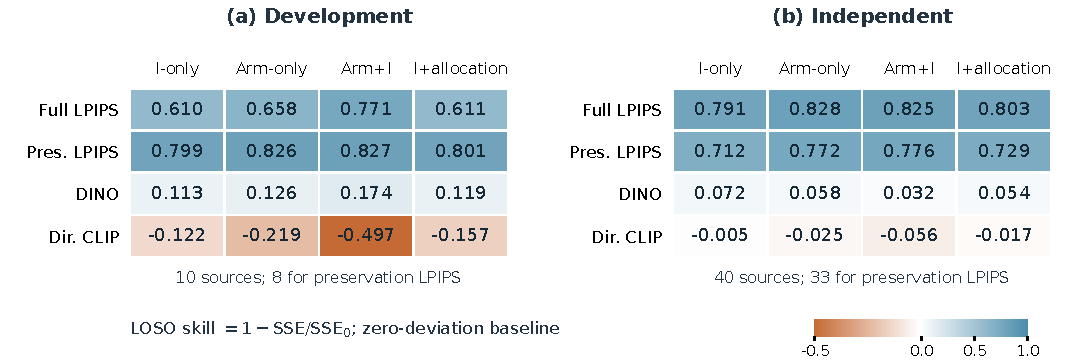
\includegraphics[width=\textwidth]{figures/LOSO_impulse_vs_allocation.pdf}
\caption{Four exploratory source-centered LOSO models: $I$ only, arm identity only, arm identity plus $I$, and $I$ plus allocation. Development (R84) and independent (R85) populations are fitted separately: $n=10/40$ sources, or $8/33$ for preservation LPIPS. Seeds are averaged within source. Points show skill $1-\mathrm{SSE}/\mathrm{SSE}_0$ against zero deviation. Held-out outcome means define scored deviations; model fitting uses training sources.}
\label{fig:doselosoprofiles}
\end{figure*}

\paragraph{Metric agreement.}
For each source, we compute Spearman correlations across the seven arm means, reversing LPIPS/MAE signs so that larger values consistently denote retention. Independent mean within-source correlation is 0.600 for DINO/negative full LPIPS (pointwise 95\% source-bootstrap interval $[0.499,0.690]$) and 0.930 for full/preservation LPIPS ($[0.902,0.955]$). Directional CLIP versus DINO averages $-0.187$ ($[-0.330,-0.045]$). Full-image associations use 40 sources and regional associations 33. Intervals use 2,000 source resamples (seed 20261103) and are pointwise and exploratory. These associations depend on the included operating points and do not establish agreement with human perception.

U25 has higher mean DINO and lower mean full/preservation LPIPS than CORR25. At source level, DINO and full-LPIPS contrast signs disagree on eight of 40 sources; DINO and preservation-LPIPS signs disagree on six of 33. The evidence supports aggregate retention-metric agreement, with source-specific disagreements rather than an established three-metric contradiction. The archived raw and centered scatter plots, residuals, and model variants preserve that distinction.

\paragraph{Request-map localization diagnostic: not yet computed.}
The inspected R85 archives retain only JPEG previews quantized from $64\times64$ response/protection maps; the protection preview is enlarged to $320\times320$. Native floating-point $E/P$ arrays are absent. The full 40-source localization contrast $L=\operatorname{mean}_{\rm edit}(E)-\operatorname{mean}_{\rm preserve}(E)$ remains unavailable from these archives. The ten-source realized-profile follow-up records regenerated native maps and a separate localization diagnostic (Section~\ref{sec:r86-details}). Exact evaluation requires saved native floating-point maps and official evaluation regions. Such map logging supports a post-hoc localization diagnostic, separate from the completed dose-profile analyses.

\paragraph{Operational consequence.}
Report the full applied-RMS sequence as well as $I$ and the nominal coefficient. Equal cumulative magnitude need not imply equal timing, direction, net latent displacement, or target-field feedback. For a strict amplitude-controlled spatial experiment, freeze a source/seed-specific profile $b_i$ and apply $\widehat c_i=\beta b_iq_i/\operatorname{RMS}(q_i)$ to each direction rule, with the same time grid and memory. Uniform, request-weighted, and displaced-map directions then receive identical step magnitudes at each chosen $\beta$. The completed realized-profile follow-up implements this intervention (Section~\ref{sec:r86-details}).

